\chapter{Introducción}




% \begin{tblr}{|Q[h,t]|Q[c,t]|Q[r,b]|}
% \hline
% {C[Au].c1ccc(cc1)P(c2ccccc2)c3ccccc3 \\ Left Left} & Middle Center & {\includegraphics{imagenes/SciFinder/Chloro[(1,1-biphenyl-2-yl)di-tert-butylphosphine]gold(I).png}} \\
% \hline
% \end{tblr}

La Química estudia la composición y estructura de la materia, sus propiedades y transformaciones. Estudia las sustancias, la energía y sus cambios durante las reacciones. Desde que se tienen registros, la química ha sido fundamental para el desarrollo de la humanidad, ya que ha permitido la producción de materiales, alimentos, medicamentos y energía, entre otros. Esto ha sido un proceso lento y exhaustivo a través de la experimentación. Por ejemplo, en 1881, Beilstein publica su Manual de Química Orgánica, que recogía 15000 compuestos orgánicos con sus propiedades \cite{handbook_1881}. Conforme la química se iba expandiendo, también lo hacía el volumen de datos que se generaban, siendo cada vez mas frecuentes preguntas como "¿alguien habrá sintetizado ya este compuesto?" \cite{applied_chemo_intro}

Eventualmente, hace unas cuantas décadas, se pensó que la cantidad de información que cada químico por su cuenta había acumulado, se podía compartir y hacer accesible a la comunidad científica a través de su almacenamiento en bases de datos \cite{chemo_a_textbook}. Con el desarrollo de técnicas de manipulación y tratamiento de esos datos surgió el término \emph{chemoinformatics}.

Las \emph{chemoinformatics} han cobrado gran importancia en los últimos años debido al aumento exponencial de datos experimentales generados en la investigación biomédica y química, y a la necesidad de manejar y analizar esta información de manera eficiente.
Esta disciplina ha sido influenciada por diversas áreas, como la química, matemáticas, estadística, biología y ciencias de la computación entre otras. Al parecer, su origen se remonta a la década de 1940, habiendo ya algunas investigaciones en el área, pero el término 'chemoinformatics' como tal se lleva utilizado más bien poco (1998) \cite{leach_introduction_2007}. Como tal, aun no hay un acuerdo en cuanto a su definición, seguramente por su carácter interdisciplinar, ni si quiera en cómo deletrearlo, pudiendo aparecer también como \emph{cheminformatics}, \emph{chemical informatics}, \emph{chemi-informatics}, y \emph{molecular informatics} entre otras \cite{leach_introduction_2007, brown_chemoinformaticsintroduction_2009}. En la literatura se discuten varias interpretaciones sobre su definición, unas más precisas y otras más generales: \cite{leach_introduction_2007, basic_overview_chemo, brown_chemoinformaticsintroduction_2009, chemo_a_textbook}


\begin{center}
\small
\textit{La mezcla de recursos de información para transformar datos en información, y la información en conocimiento, con el fin de tomar decisiones más rápidas y efectivas en la identificación y optimización de fármacos} [Brown 1998]
\end{center}

\begin{center}
\small
\textit{Chem(o)informatics es un término genérico que abarca el diseño, la creación, la organización, la gestión, la recuperación, el análisis, la difusión, la visualización y el uso de la información química. }[G. Paris 1999]
\end{center}

\begin{center}
\small
\textit{La aplicación de métodos informáticos para resolver problemas de química} [J. Gasteiger and T. Engel 2006]
\end{center}


A pesar de ello, son a día de hoy un componente esencial en el descubrimiento de sustancias químicas; sin duda es un área en constante evolución y su importancia solo aumentará en los próximos años, tanto en el descubrimiento de fármacos —que es como originariamente surgió y donde más impacto tiene en la sociedad— como en otros campos de la química.


Una herramienta también de vital importancia en este ámbito son los sistemas de representación lineal. Surgieron a medida que la química y la tecnología computacional avanzaban, y nos permiten codificar moléculas para su análisis y almacenamiento en bases de datos. En el siglo XIX, se desarrollaron varias formas de representación visual de moléculas, como las fórmulas estructurales que permitieron a los químicos dibujar y visualizar moléculas de manera más efectiva. Sin embargo, estas formas de representación no son adecuadas para su uso en la computación, ya que no son fácilmente legibles para los programas informáticos. Nosotros, los humanos, cuando vemos una estructura molecular dibujada la entendemos directamente, obtenemos una visión global de los símbolos que representan los enlaces y la distribución espacial de los átomos que la componen, pero los computadores no tienen esa facilidad. Por ello, se desarrollaron sistemas de notación lineal que permitían describir de manera más precisa y eficiente la estructura molecular, trabajando con tipos de datos sencillos, cadenas de caracteres.


\section{Motivación y objetivos}

Los formatos de notación lineal llevan siendo un tema de interés e investigación para los científicos desde mediados del siglo 19, evolucionando poco a poco y desarrollándose nuevas notaciones en función de las necesidades —principalmente computacionales— del momento y las limitaciones que se iban descubriendo \cite{107_years_linear_notations}. En la actualidad, existen varias representaciones lineales, siendo las más usadas SMILES, InChI, y SELFIES \cite{SELFIES}. Como comenté antes, una forma muy potente de representar moléculas y compuestos químicos es mediante cadenas strings, y de esto justamente se encargan las representaciones lineales: traducir una molécula, con sus átomos, enlaces entre ellos, ciclos y otras propiedades características, en una cadena string que la represente, y que la máquina y los propios químicos puedan entender. Sin embargo, hay diferencias notables entre las representaciones, tanto en la sintaxis de las cadenas que se generan como en las aplicaciones que se le puede dar a cada una de ellas.


SMILES, ideada por David Weininger, sale a la luz en 1988 satisfaciendo con creces las necesidades de procesamiento de información química que había, desbancando a la representación estandarizada del momento, Wiswesser Line Notation (WLN). Desde ese entonces SMILES se convirtió —y sigue siendo a día de hoy— en el estándar de representación lineal, ya que permite describir estructuras moleculares de una forma sencilla en un formato fácil de leer, lo que ha hecho que sea una herramienta popular en la química computacional, siendo la más usada entre investigadores y químicos. Pese a esto, SMILES tiene dos grandes inconvenientes: una misma molécula puede escribirse con varias cadenas SMILES distintas válidas, es decir, tiene sinónimos (Figura \ref{fig:sinonimos_smiles}); y no es robusto ni sintáctica ni semánticamente. En este sentido se podría generar un string que no represente una molécula válida, como lo es \emph{CC(CCCC}, el cual tiene un paréntesis sin cerrar (lo que implica que no se delimita cuándo acaba la rama). O generar una molécula que no sea químicamente viable como \emph{CO=CC}, que muestra un átomo de oxígeno neutro formando tres enlaces (superando el límite de enlaces covalentes que un oxígeno neutro puede tener) \cite{SELFIES}.

\begin{figure}[H]
\centering
    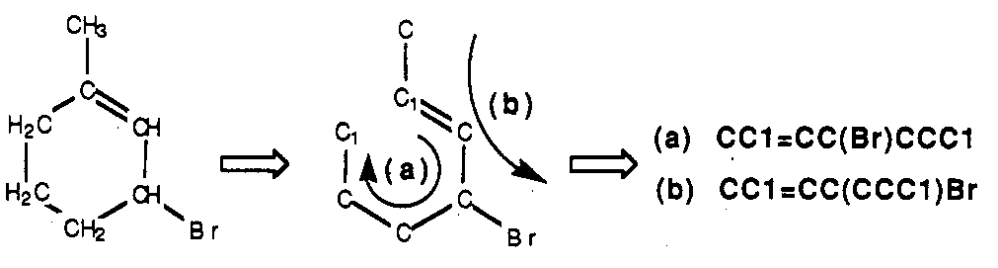
\includegraphics[scale=0.4]{imagenes/intro/sinonimos.png}
    \caption{Distintas cadenas SMILES válidas para el 1-methyl-3-bromo-ciclohexeno. \textbf{(a)} Considera el ciclo como la rama principal y el bromo como ramificación. \textbf{(b)} Hace el recorrido que marca la flecha, dejando parte del ciclo como una ramificación. Imagen extraída de \cite{weininger_smiles_1988}}
    \label{fig:sinonimos_smiles}
\end{figure}

Esto tiene especial relevancia en el ámbito del Machine Learning (ML). Aunque se sale del alcance de este trabajo, uno de los grandes objetivos de la química computacional es la creación o diseño de nuevas moléculas. Se podrían crear modelos de ML o redes neuronales capaces de generar moléculas ficticias válidas, para posteriormente ver sus propiedades, valorarlas energéticamente para ver cuán estables son, y estudiar su viabilidad en distintas aplicaciones, entre otras cosas. SMILES dificulta esta tarea, y por ello, aparece en 2020, SELFIES (SELF-referencIng Embedded Strings), una nueva representación lineal 100\% robusta, muy usada actualmente para modelos generativos. Ver \cite{SELFIES, krenn_self_referencing_2020} para más detalles de cómo soluciona los problemas de robustez y otras características de la representación. SELFIES es relativamente reciente y continuamente está ampliando sus funcionalidades, mejorando su simplicidad y facilidad de uso para el usuario \cite{selfies_recent_2023}. Aun así, no se termina de instaurar entre la comunidad investigadora. Por último, InChI es creado en 2013 por la IUPAC (International Union of Pure and Applied Chemistry) como un proyecto para estandarizar el proceso de búsqueda de estructuras moleculares entre distintas bases de datos. Esto es porque InChI (International Chemical Identifier) genera una cadena canónica única para cada molécula, de manera que cada molécula tiene una sola representación, y dicha representación solamente hace referencia a esa molécula. La principal desventaja radica en su sintaxis y su estructura jerárquica, haciéndola complicada de leer y utilizar por los humanos. Por esto mismo también, no es la mejor opción para usar en modelos generativos, pues tiene una serie de reglas y normas gramaticales y aritméticas que son complejas de aplicar al generar moléculas a través de modelos de ML.\cite{heller_inchi_2015}


Por todo lo anterior, me centraré en la notación SMILES durante el desarrollo de este trabajo. Dicho esto, existen diversas bases de datos en química donde se recoge gran cantidad de información acerca de los compuestos. Entiéndase esto como una colección estructurada y organizada que contiene datos sobre compuestos químicos, sus propiedades y relaciones con otros compuestos. Se utilizan para almacenar y recuperar información sobre moléculas, sustancias, reacciones, propiedades fisicoquímicas, e incluso literatura científica relacionada. Menciono las más importantes y las que serán objeto de interés. \emph{PubChem}, una base de datos abierta que sirve información a millones de usuarios en todo el mundo, desde investigadores y estudiantes hasta el público general. Recogen para cada compuesto, información sobre su estructura, representaciones 2D y 3D, identificadores, propiedades químicas y físicas, patentes, avisos de toxicidad, etc. \cite{pubchem_website} 


\begin{table}[h!]
\small
\centering
    \begin{tabular}{m{7cm}>{\centering\arraybackslash}m{4cm}}
        \hline
        \textbf{Código SMILES} & \textbf{Representación 2D} \\
        \hline
        C[Au].c1ccc(cc1)P(c2ccccc2)c3ccccc3 & 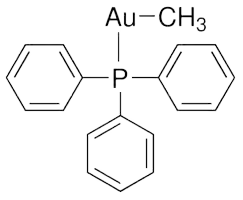
\includegraphics[width=2.2cm]{imagenes/sigmaAldrich/Methyl(triphenylphosphine)gold(I)} \\ [0.8cm]
        \hline
        Cl[Pd]Cl.C1CC=CCCC=C1 & 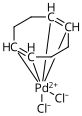
\includegraphics[width=2.2cm]{imagenes/sigmaAldrich/Dichloro(1,5-cyclooctadiene)palladium(II).png} \\ 
        \hline
        Cl[Au].CP(C)C & 
\includegraphics[width=2.2cm]{imagenes/sigmaAldrich/Chloro(trimethylphosphine)gold(I).png} \\ [0.8cm]
        \hline
         Cl[Au].CC(C)(C)P(c1ccccc1-c2ccccc2)C(C)(C)C & \includegraphics[width=2.2cm]{imagenes/sigmaAldrich/Chloro[(1,1-biphenyl-2-yl)di-tert-butylphosphine]gold(I).png} \\
        \hline
        [Fe]I.[C-]\#[O+].[C-]\#[O+].[CH]1[CH][CH][CH][CH]1 & 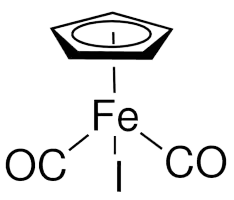
\includegraphics[width=2.2cm]{imagenes/sigmaAldrich/Dicarbonylcyclopentadienyliodoiron(II).png} \\
        \hline
        % Br[Ni]Br.COCCOC & \includegraphics[width=2.2cm]{imagenes/sigmaAldrich/Nickel(II) bromide ethylene glycol dimethyl ether complex.png} \\
        % \hline
        \end{tabular}
    \caption{Códigos SMILES y sus representaciones visuales según Sigma-Aldrich}
    \label{tabla:tabla_peq_intro_sigmaAldrich}
\end{table}

\emph{SciFinder}, una herramienta de investigación muy potente que permite explorar las bases de datos de CAS (American Chemical Society) las cuales contienen literatura sobre Química y otras disciplinas afines como Física, Biomedicina, Geología, Ingeniería Química, etc. Incluye referencias bibliográficas y resúmenes de artículos, informes, y libros entre otras cosas. Permite realizar búsquedas por estructura, nombres de sustancias o identificadores, reacciones en la que participa dicha sustancia, artículos y publicaciones que nombren el compuesto en cuestión, e incluso proveedores de compra \cite{scifinder_website}. Para el uso de esta herramienta es necesario acceder mediante la red de una institución autorizada (en este caso trabajo mediante VPN de la UGR) y seguir los pasos para registrarte \footnote{Pasos para el registro en SciFinder \url{https://bibliotecaugr.libguides.com/scifinder_scholar}}. Y \emph{Sigma-Aldrich}, una compañía de ciencia, química y biotecnología que se dedica a la producción y venta de productos químicos, reactivos, equipos y materiales de laboratorio. Ofrece herramientas, servicios, artículos y una gran variedad de productos químicos que se utilizan en investigación, biofarmacéutica, e industria entre otros ámbitos \cite{sigma_aldrich_web}. A través de su página web se enfocan al comercio electrónico pudiendo buscar y comprar productos, compuestos orgánicos e inorgánicos, agentes reactivos, isótopos para síntesis químicas, proteínas, enzimas, etc. De cada producto muestra información relevante como la ficha de datos de seguridad, detalles de las propiedades físicas y químicas así como algunas representaciones lineales del compuesto y la representación del grafo molecular, que es lo interesante en este caso realmente.





\begin{table}[h!]
\small
\centering
    \begin{tabular}{m{7cm}>{\centering\arraybackslash}m{4cm}}
        \hline
        \textbf{Código SMILES} & \textbf{Representación 2D} \\
        \hline
        [Au+]([CH3-])[P](C=1C=CC=CC1) (C=2C=CC=CC2)C=3C=CC=CC3 & 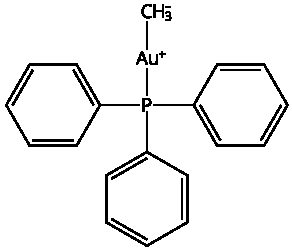
\includegraphics[width=2.2cm]{imagenes/sciFinder/pdf/Methyl(triphenylphosphine)gold(I).pdf} \\
        \hline
        [Cl-][Pd+2]123([Cl-]) [CH]=4CC[CH]3=[CH]2CC[CH]41 & 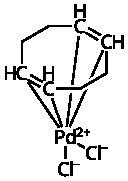
\includegraphics[width=2.2cm]{imagenes/sciFinder/pdf/Dichloro(1,5-cyclooctadiene)palladium(II).pdf} \\
        \hline
        [Cl-][Au+][P](C)(C)C & 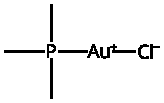
\includegraphics[width=2.2cm]{imagenes/sciFinder/pdf/Chloro(trimethylphosphine)gold(I).pdf} \\
        \hline
        [Cl-][Au+][P](C=1C=CC=CC1C=2C=CC=CC2) (C(C)(C)C)C(C)(C)C & 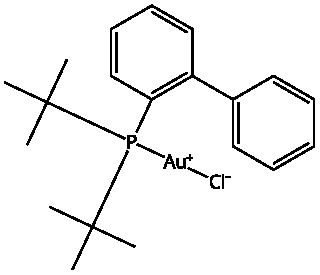
\includegraphics[width=2.2cm]{imagenes/sciFinder/pdf/Chloro[(1,1-biphenyl-2-yl)di-tert-butylphosphine]gold(I).pdf} \\
        \hline
        O\#C[Fe+2]1234([I-])(C\#O)[CH]=5[CH]4 =[CH]3[CH-]2[CH]51 & 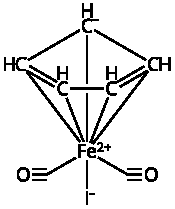
\includegraphics[width=2.2cm]{imagenes/sciFinder/pdf/Dicarbonylcyclopentadienyliodoiron(II).pdf} \\
        \hline
        % [Br-][Ni+2]1([Br-])O(C)CCO1C & \includegraphics[width=2.2cm]{imagenes/sciFinder/Nickel(II) bromide ethylene glycol dimethyl ether complex.png} \\
        % \hline
        \end{tabular}
    \caption{Códigos SMILES y sus representaciones visuales según SciFinder}
    \label{tabla:tabla_peq_intro_sciFinder}
\end{table}


Desde la Universidad de Granada, la tutora de este TFG colabora el grupo de investigación de químicos del ICIQ (Instituto Catalán de Investigación Química) liderado por la profesora Mónica H. Pérez-Temprano. Su foco de investigación gira en torno al entendimiento de transformaciones catalíticas en las que participan compuestos organometálicos, descubriendo y diseñando reacciones más eficientes basadas en catalizadores metálicos. Para más detalle sobre el grupo de investigación y sus ámbitos de trabajo, ver su sitio web \cite{ICIQ}. En resumen, intentan desarrollar enfoques más sostenibles para la síntesis de moléculas orgánicas usando la química organometálica. Como tal, necesitan codificar correctamente una molécula de organometálica en pos de trabajar con ella adecuadamente y utilizar todas las herramientas, para, entre otras cosas, poder dibujarla y entenderla mejor.


Uno de los principales problemas que se detectan es la heterogeneidad en las distintas bases de datos para un mismo compuesto o molécula. Para ilustrar esto, presento las tablas \ref{tabla:tabla_peq_intro_sigmaAldrich} y \ref{tabla:tabla_peq_intro_sciFinder}. Ambas tablas comparan las mismas moléculas, mostrando el código SMILES y la representación visual que ofrecen las bases de datos Sigma-Aldrich y SciFinder respectivamente. Vemos diferencias claras en el tratamiento de los ciclos aromáticos, la especificación de las cargas de los átomos y la posición de algunas ramificaciones. Utilizo un subset de 5 moléculas pertenecientes a la organometálica, seleccionadas desde un conjunto de datos de 30 moléculas considerados de interés por los químicos con los que colabora la tutora (disponible para su consulta en mi GitHub \footnote{\url{https://github.com/Jesnm01/TFG}}). En el Apéndice \ref{apend:tabla_intro_grande}, se puede consultar una tabla comparativa con el set de moléculas al completo. 














\section{Objetivos}
Por tanto, el objetivo principal de este Trabajo Fin de Grado sería modificar el paquete OpenBabel creando un método para canonizar códigos SMILES, orientado específicamente para compuestos organometálicos. Para ello, se establecen los siguientes subobjetivos:
\begin{itemize}
    \item Analizar y comparar las cadenas SMILES de distintas bases de datos (p.ej. Sigma-Aldrich, SciFinder) viendo los posibles sinónimos para una misma molécula.
    \item Determinar un sistema que genere, a partir de cualquier sinónimo SMILES de la misma molécula, un único SMILES canónico.
    \item Definir otro algoritmo o conjunto de reglas que mejore, aunque sea mínimamente, el sistema de dibujado de las moléculas.
\end{itemize} 

\section{Estructura de la memoria}
\textbf{esperar a tenerla mas avanzada para completar esto}






% \begin{longtable}{|c|>{\centering\arraybackslash}b{3cm}|m{3cm}|c|c|}
% \caption{Título de la tabla} \\
% \hline
% \textbf{Columna 1} & \textbf{Columna 2} & \textbf{Columna 3} & \textbf{Columna 4} & \textbf{Columna 5} \\ \hline
% \endfirsthead

% \multicolumn{5}{c}%
% {{\bfseries \tablename\ \thetable{} -- Continuación de la tabla}} \\
% \hline
% \textbf{Columna 1} & \textbf{Columna 2} & \textbf{Columna 3} & \textbf{Columna 4} & \textbf{Columna 5} \\ \hline
% \endhead

% \hline \multicolumn{5}{r}{\textit{Continúa en la siguiente página}} \\
% \endfoot

% \hline
% \endlastfoot

% Fila 1, Columna 1 & [Au+]([CH3-])[P](C=1C=CC=CC1) (C=2C=CC=CC2)C=3C=CC=CC3  & Fila 1, Columna 3 & Fila 1, Columna 4 & 
\includegraphics[width=2.2cm]{imagenes/sciFinder/Chloro(trimethylphosphine)gold(I).png} \\ \midrule
% Fila 1, Columna 1 & Fila 1, Columna 2 & Fila 1, Columna 3 & Fila 1, Columna 4 & 
\includegraphics[width=2.2cm]{imagenes/sciFinder/Chloro(trimethylphosphine)gold(I).png} \\ \hline
% Fila 1, Columna 1 & Fila 1, Columna 2 & Fila 1, Columna 3 & Fila 1, Columna 4 & 
\includegraphics[width=2.2cm]{imagenes/sciFinder/Chloro(trimethylphosphine)gold(I).png} \\ \hline
% Fila 1, Columna 1 & Fila 1, Columna 2 & Fila 1, Columna 3 & Fila 1, Columna 4 & 
\includegraphics[width=2.2cm]{imagenes/sciFinder/Chloro(trimethylphosphine)gold(I).png} \\ \hline

% \end{longtable}
